\chapter{Etude de la cascade turbulente dans un plasma incompressible}
\renewcommand\partie{\Partie\ Chapitre \thechapter}
\label{ch-11}

%\medskip
\minitoc  

\bigskip

Ce n'est que 57 ans après l'apport de Kolmogorov à la compréhension de la turbulence que l'idée de chercher des lois exactes dans un fluide magnétisé, ou plasma, a émergé. Ainsi, \cite{politano_von_1998} et \cite{politano_dynamical_1998} ont étendu la théorie hydrodynamique à la \ac{MHD} en restant dans le cadre incompressible. Cette avancée historique a apporté un cadre à l'étude de la turbulence dans les plasmas spatiaux. Dans le laboratoire qu'est le vent solaire, elle a permis de trouver des éléments de réponse à des problèmes tels que ceux du chauffage ou de l'accélération du vent [\cite{smith_dependence_2006,sorriso-valvo_observation_2007,stawarz_turbulent_2009,osman_proton_2013,bruno_solar_2013,alexandrova_solar_2013,sahraoui_magnetohydrodynamic_2020,marino_scaling_2023}]. 

Le modèle incompressible magnétohydrodynamique idéal avec pression isotrope (\acs{IMHD}) est la description fluide d'un plasma la plus simple abordée dans ce mémoire. Dans ce chapitre, nous reprendrons les résultats analytiques incompressibles principaux afin d'introduire les outils fondamentaux de l'étude de la turbulence dans un plasma.

\section{Le modèle et l'énergie totale}
\label{sec-111}
Contrairement au modèle hydrodynamique incompressible abordé dans le Chapitre \ref{ch-01}, dans le cas d'un plasma, il est nécessaire de prendre en compte le couplage entre le fluide et le champ magnétique et d'ajouter l'équation d'induction \eqref{eq:synth_M3_ideal} comme on a pu le mettre en pratique dans le Chapitre \ref{ch-02}. L'incompressibilité s'exprime quant à elle à travers la contrainte $\nabla \cdot \boldsymbol{v} = 0$. Le modèle magnétohydrodynamique incompressible (\acs{IMHD}) est alors :
\begin{eqnarray}
\label{eq:model_inc_v} \partial_t \boldsymbol{v} + \boldsymbol{v} \cdot \nabla \boldsymbol{v} -  \boldsymbol{v_A} \cdot \nabla \boldsymbol{v_A} + \frac{1}{\rho_0} \nabla p_* &=& 0, \\
\label{eq:model_inc_b} \partial_t \boldsymbol{v_A} + \boldsymbol{v} \cdot \nabla \boldsymbol{v_A} -  \boldsymbol{v_A} \cdot \nabla \boldsymbol{v}&=& 0, \\
\label{eq:model_inc_r} \nabla \cdot \boldsymbol{v} &=& 0.
\end{eqnarray}
Le champ magnétique apparaît dans ces équations à travers la vitesse d'Alfvén $\boldsymbol{v_A} = \boldsymbol{B}/\sqrt{\mu_0 \rho_0}$ et la pression magnétique $p_m = \rho_0 \boldsymbol{v_A}^2 /2$ contenue dans la pression totale $p_* = p + p_m$. On remarque qu'il y a 3 équations (7 en termes de composantes) et 3 inconnues (2 vectorielles, $\boldsymbol{v}$ et $\boldsymbol{v_A}$ et une scalaire, $p$). Le système se retrouve donc fermé grâce à la contrainte incompressible en équation \eqref{eq:model_inc_r}. On peut rappeler aussi que le champ magnétique est aussi contraint tel que $\nabla \cdot \boldsymbol{B} = 0$, ce qui implique dans le cas incompressible : $\nabla \cdot \boldsymbol{v_A} = 0$ (contrainte implicitement prise en compte dans l'équation d'induction \eqref{eq:model_inc_b}). En appliquant la divergence sur l'équation \eqref{eq:model_inc_v}, on obtient l'équilibre de pression, $- \frac{1}{\rho_0}\nabla^2 p_* = \nabla \boldsymbol{v} : \nabla \boldsymbol{v} -  \nabla \boldsymbol{v_A} : \nabla \boldsymbol{v_A} $, qui indique que la pression totale est directement reliée aux non-linéarités du système.\footnote{Ce système peut aussi être symétrisé grâce aux variables d'Elsässer, $\boldsymbol{z^{\pm}} = \boldsymbol{v} \pm \boldsymbol{v_A}$: 
\begin{eqnarray}
\partial_t \boldsymbol{z^{\pm}} + \boldsymbol{z^{\mp}} \cdot \nabla \boldsymbol{z^{\pm}} = - \frac{1}{\rho_0} \nabla p_* , &\qquad& \nabla \cdot \boldsymbol{z^{\pm}} = 0 .
\end{eqnarray}
Leur somme $\frac{1}{4}\rho_0 (\boldsymbol{z^{+}}{}^2 + \boldsymbol{z^{-}}{}^2)$ donne l'énergie totale $E_{tot}$ et leur différence, l'hélicité croisée  $H_c$. La dynamique non-linéaire est alors contenue dans le terme $\boldsymbol{z^{\mp}} \cdot \nabla \boldsymbol{z^{\pm}}$. De telles variables sont adaptées à l'étude de ce système incompressible et sont largement utilisées pour simplifier les calculs. Il est nécessaire de garder en tête qu'en termes de mathématique fondamentale, elles ne peuvent exister, car elles sont la somme d'un champ vectoriel (vitesse) et d'un champ pseudo-vectoriel (champ magnétique). Dans un effort de cohérence avec le cadre compressible dans lequel elles sont mal définies [\cite{magyar_nature_2019}], elles ne seront pas utilisées ici.}

Dans ce système apparaissent deux canaux énergétiques : cinétique de densité $E_c = \frac{1}{2} \rho_0 \boldsymbol{v}^2$, et magnétique, $E_m = \frac{1}{2} \rho_0 \boldsymbol{v_A}^2$. On définit aussi la densité d'hélicité croisée couplant les deux champs : $H_c = \rho_0 \boldsymbol{v_A} \cdot \boldsymbol{v}$. Les équations de densité d'énergie cinétique et magnétique, obtenue respectivement à partir de \eqref{eq:model_inc_v} et  \eqref{eq:model_inc_b}, et celle de densité d'énergie totale $E_{tot} = E_c + E_m$ sont alors : 
\begin{eqnarray}
 \label{eq:model_inc_k} \partial_t E_c +   \nabla  \cdot (E_c \boldsymbol{v}+ H_c \boldsymbol{v_A} + p_* \boldsymbol{v}  )  &=& - \rho_0  \boldsymbol{v_A} \boldsymbol{v_A} : \nabla \boldsymbol{v}, \\
 \label{eq:model_inc_m} \partial_t E_m +   \nabla  \cdot (E_m \boldsymbol{v}) &=& \rho_0   \boldsymbol{v_A} \boldsymbol{v_A} : \nabla \boldsymbol{v} ,\\
\label{eq:model_inc_e} \partial_t E_{tot} +   \nabla  \cdot (E_{tot} \boldsymbol{v} + H_c \boldsymbol{v_A} + p_* \boldsymbol{v} )  &=&  0.
\end{eqnarray}
L'équation \eqref{eq:model_inc_e} indique que la densité d'énergie totale moyenne $\left<E_{tot}\right>$ est conservée puisque pour toute quantité $\boldsymbol{X}$, la moyenne, ici spatiale, $\left<\right>$, implique\footnote{En supposant la périodicité de $\boldsymbol{X}$ ou son annulation à l'infinie.} $\left<\nabla \cdot \boldsymbol{X}\right> = 0$. Les équations \eqref{eq:model_inc_k} et \eqref{eq:model_inc_m} nous indiquent un échange entre les canaux énergétiques se faisant à travers le terme de droite. 

\section{Le cas linéaire et les ondes d'Alfvén}
La théorie linéaire est la principale voie nous donnant des informations ondulatoires sur un modèle. Ainsi, dans le modèle \acs{IMHD}, elle vient révéler l'existence des ondes dites d'Alfvén. 

Pour cela, on doit linéariser le système, c'est-à-dire négliger tout terme non-linéaire (d'ordre supérieur à 1). 
Les moyennes des quantités impliquées seront indiquée par un 0 (ordre 0) et les fluctuations d'ordre 1 seront indiquées par un 1. Ainsi, par exemple, $\boldsymbol{v} \simeq \boldsymbol{v_{0}} + \boldsymbol{v_{1}}$. On considèrera aussi que $\boldsymbol{v_{0}} = 0$ et on notera la direction du champ magnétique moyen $\boldsymbol{b_0}$. 

\label{sec-112}
\begin{wrapfigure}{r}{0.5\textwidth}
 \centering
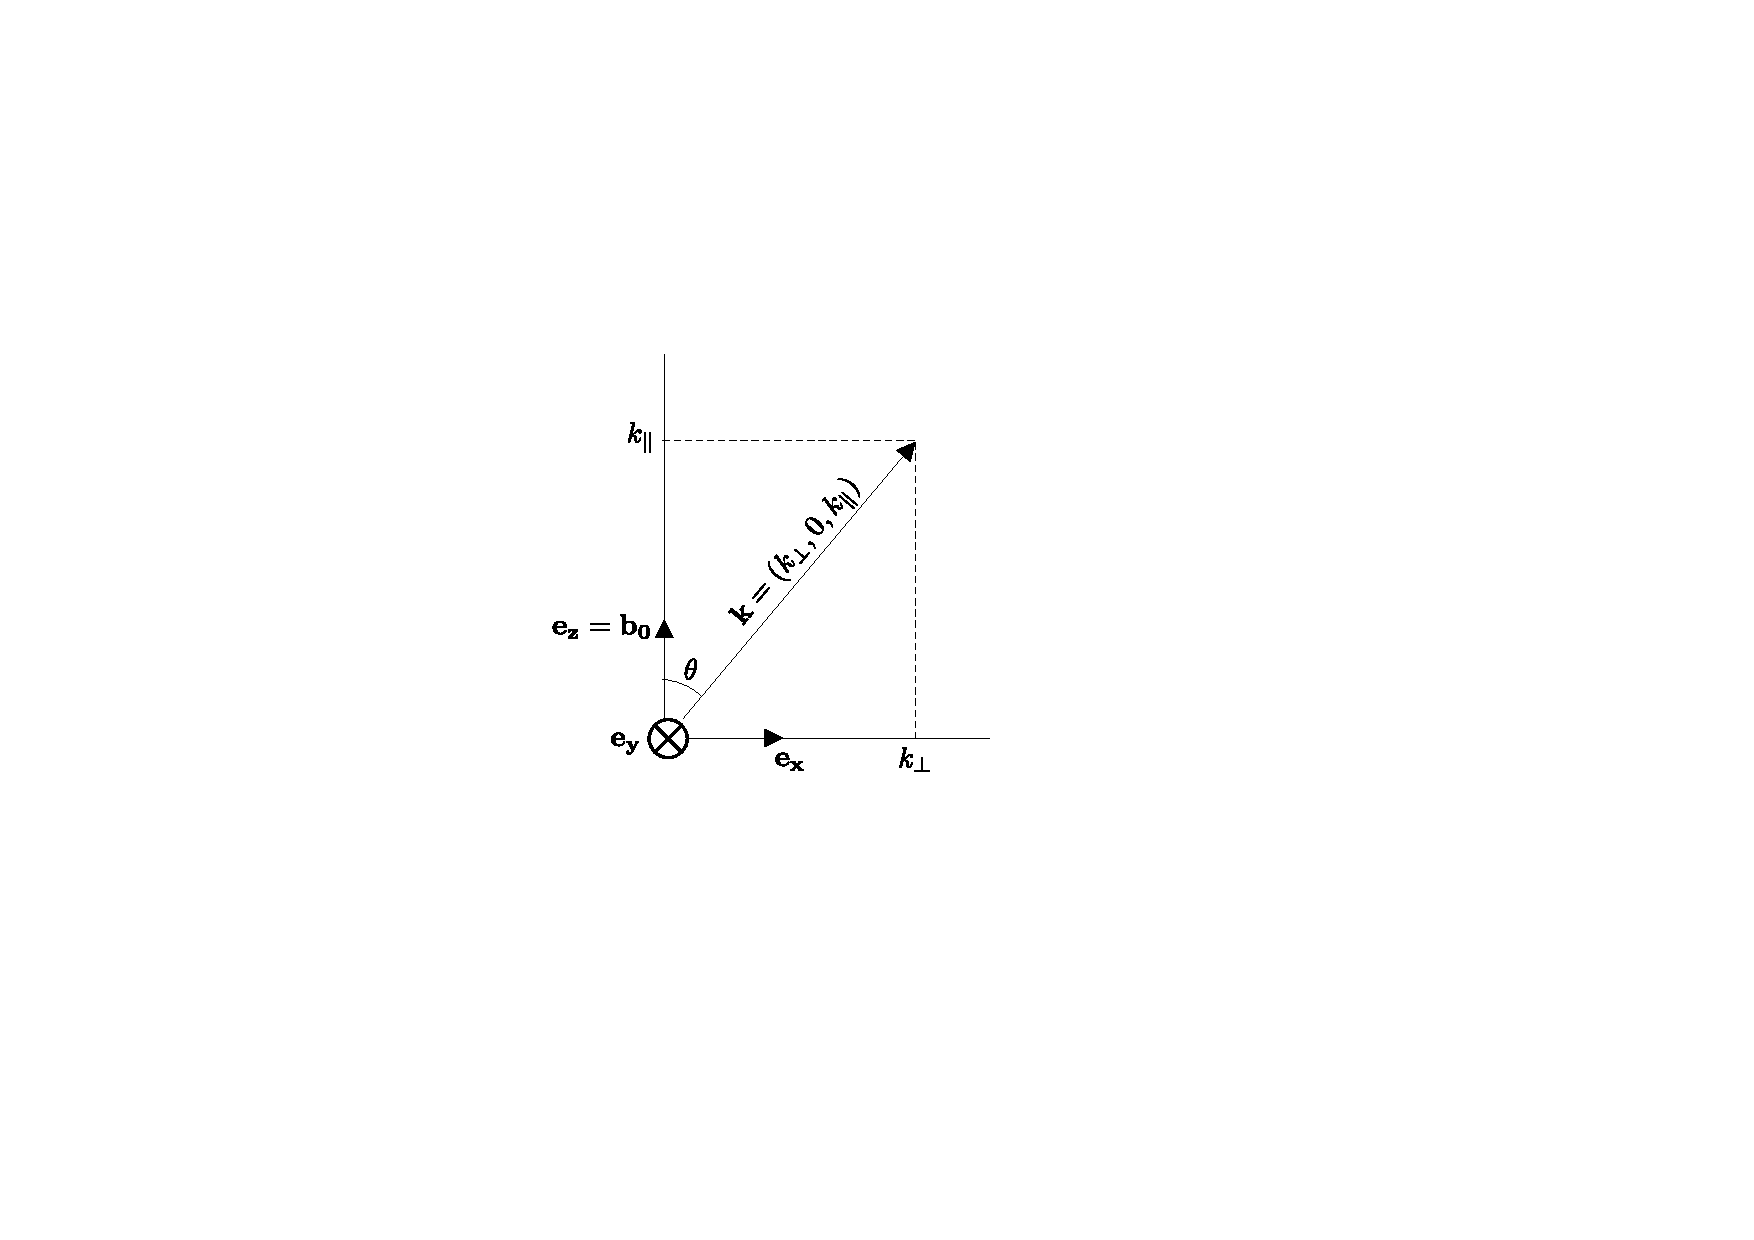
\includegraphics[width=0.6\linewidth,trim=9.3cm 7.8cm 13cm 7cm, clip=true]{./Part_1/images/schema_kplan.pdf}
\caption{Système de coordonnées et vecteur d'onde dans le cadre linéaire.}
\label{fig:schema_kplan}
\end{wrapfigure}

La deuxième étape consiste à passer dans l'espace de Fourier, c'est-à-dire remplacer $\partial_t$ par la pulsation $-i\omega$ et $\nabla$ par le vecteur d'onde $i\boldsymbol{k}$. On supposera sans perte de généralité, le système de coordonnées cartésiennes orienté tel que $\boldsymbol{e_z} = \boldsymbol{b_0}$ et la composante suivant $\boldsymbol{e_y}$ du vecteur d'onde, $k_y = 0$. On notera $k$ la norme du vecteur d'onde, $k_{\parallel}$ sa composante le long de $\boldsymbol{e_z}$, parallèle au champ magnétique moyen, $k_{\perp}$ sa composante le long de $\boldsymbol{e_x}$ et $\theta$ l'angle formé avec $\boldsymbol{e_z}$ (voir \figref{fig:schema_kplan}).
Le système \acs{IMHD} devient alors : 
\begin{eqnarray}
 \label{eq:lin_inc_v} \omega \boldsymbol{v_{1}}  + v_{A0} k_{\parallel} \boldsymbol{v_{A1}} - \frac{1}{\rho_0}  p_{*1} \boldsymbol{k}&=& 0 ,\\
 \label{eq:lin_inc_b} \omega \boldsymbol{v_{A1}}  +  v_{A0} k_{\parallel}  \boldsymbol{v_{1}}&=& 0 ,\\
 \label{eq:lin_inc_r} \boldsymbol{k} \cdot \boldsymbol{v_{1}} = 0 \qquad \boldsymbol{k} \cdot \boldsymbol{v_{A1}}  &=& 0 .
\end{eqnarray}

Ensuite, on injecte les équations \eqref{eq:lin_inc_b} et \eqref{eq:lin_inc_r} dans l'équation \eqref{eq:lin_inc_v} : 
\begin{itemize}
    \item $\boldsymbol{k} \cdot \eqref{eq:lin_inc_v} \Rightarrow  p_{*1} =0$, en excluant le cas trivial où $\boldsymbol{k}=0$. La pression totale n'est donc bien reliée qu'aux non-linéarités du système.
    \item $\omega \cdot \eqref{eq:lin_inc_v} \Rightarrow (\omega^2   - (\boldsymbol{k} \cdot \boldsymbol{v_{A0}})^2 ) \boldsymbol{v_{1}} = 0$ (dite équation de dispersion), d'où la relation de dispersion :  
    \begin{equation}
        \label{eq:lin_inc_disp} \omega = \pm \boldsymbol{k} \cdot \boldsymbol{v_{A0}} = \pm v_{A0} k_{\parallel} =  \pm v_{A0} k \cos \theta .
    \end{equation}
    \item \eqref{eq:lin_inc_b} et \eqref{eq:lin_inc_disp} $ \Rightarrow \boldsymbol{v_{1}} = \pm \boldsymbol{v_{A1}}$.
    \item $ p_{*1} =0 \Rightarrow p_{1} = - v_{A0} v_{A1z}$ .
\end{itemize}
La relation de dispersion \eqref{eq:lin_inc_disp} nous indique qu'il peut y avoir dans le système \acs{IMHD}, des ondes dites d'Alfvén, couplant champ magnétique et champ de vitesse. 
Généralement, pour obtenir la polarisation d'une onde, on injecte sa relation de dispersion dans le système. Dans le cas du système \acs{IMHD}, le système s'annule alors complètement. La polarisation de l'onde d'Alfvén dans le cas \acs{IMHD}, est définie par $\boldsymbol{k} \cdot \boldsymbol{v_{A1}}  = 0 $ qui indique que $\boldsymbol{v_{A1}} $ doit être perpendiculaire à $\boldsymbol{k}$. Or $\boldsymbol{k}$ est dans le plan $\boldsymbol{e_x}-\boldsymbol{e_z}$. Donc $\boldsymbol{v_{A1}} $ est polarisé suivant une combinaison linéaire des vecteurs $\boldsymbol{e_y}$ et $(-\cos \theta, 0, \sin \theta)$. Le mode d'Alfvén est donc dégénéré, il est formé d'un mode dit incompressible, polarisé suivant $\boldsymbol{e_y}$, et d'un mode dit pseudo-alfvénique, polarisé suivant $(-\cos \theta, 0, \sin \theta)$.

L'onde d'Alfvén est très importante en physique des plasmas, elle est, en effet, solution exacte du système \acs{IMHD} linéaire et non linéaire. En turbulence, elle peut donc alimenter la cascade. Lorsque la cascade est développée par des ondes, on parlera de turbulence d'onde. De plus, deux régimes existent :  la turbulence faible où la cascade d'énergie est supposément développée par des interactions faiblement non-linéaires entre paquets d'ondes et, la turbulence forte où ondes et structures cohérentes (de type vortex par exemple) coexistent et entretiennent la cascade. 

\section{Décrire la cascade turbulente incompressible avec une loi exacte}
\label{sec-113}
La théorie des lois exactes, nommée ainsi car aucune hypothèse de linéarisation ou perturbative n'est supposée pour les obtenir, s'appuie sur les hypothèses de Kolmogorov exposées et illustrées dans le Chapitre \ref{ch-01} (voir synthèse \ref{synt-01}) et rappelées ci-après. On se réfèrera au chapitre \ref{ch-01} à propos des notations. Historiquement, de multiples versions de la loi exacte décrivant la cascade \acs{IMHD} et de la méthode pour l'obtenir existent [\cite{politano_von_1998,galtier_origin_2018,macbride_turbulent_2008}]. On la nommera dans la suite \acs{PP98} du nom des deux chercheuses ayant dérivé la première version en 1998.

D'après les hypothèses de Kolmogorov, la zone inertielle est définie comme l'ensemble des échelles où le tranfert s'effectue conservativement. L'énergie totale (cinétique + magnétique) étant un invariant du système \acs{IMHD}, elle peut a priori cascader de manière conservative. 
Une cascade d'énergie implique une source d'injection et un canal de dissipation, respectivement aux grandes et petites échelles. Le canal de dissipation transfert l'énergie des champs électromagnétiques vers les particules du plasma. Cette énergie sera visible dans la fonction de distribution des particules à travers une augmentation de sa largeur (chauffage) ou un décalage de la moyenne (accélération). Dans le cadre \acs{IMHD}, les dissipations généralement admises sont des dissipations visqueuses ou résistives qui s'accompagnent d'une variation d'entropie. 
Le canal d'injection est nécessaire pour entretenir la cascade et compenser la dissipation dans le bilan énergétique (dans le cas incompressible) [\cite{galtier_physique_2021}]. Pour refléter cela dans les équations, on va ajouter une force $\boldsymbol{f_c}$ d'injection agissant à grande échelle et un terme dissipatif (visqueux), $\boldsymbol{d_c}$, agissant à petite échelle, dans l'équation \eqref{eq:model_inc_v} et, pour permettre la visualisation de ce que deviennent ces sources si elles sont définies magnétiquement, on va ajouter $\boldsymbol{f_m}$ et $\boldsymbol{d_m}$ (résistif) dans l'équation d'induction \eqref{eq:model_inc_b}. On restera dans un cadre général en ne détaillant pas leur contenu. Ainsi :
\begin{eqnarray}
\label{eq:turb_inc_v} \partial_t \boldsymbol{v} + \boldsymbol{v} \cdot \nabla \boldsymbol{v} -  \boldsymbol{v_A} \cdot \nabla \boldsymbol{v_A} + \frac{1}{\rho_0} \nabla p_* &=&  \boldsymbol{f_c} + \boldsymbol{d_c} , \\
\label{eq:turb_inc_b}  \partial_t \boldsymbol{v_A} + \boldsymbol{v} \cdot \nabla \boldsymbol{v_A} -  \boldsymbol{v_A} \cdot \nabla \boldsymbol{v}&=& \boldsymbol{f_m} + \boldsymbol{d_m} ,\\
\label{eq:turb_inc_r}  \nabla \cdot \boldsymbol{v} = 0, && \nabla \cdot \boldsymbol{v_A} = 0.
\end{eqnarray}

Maintenant, si l'on veut une loi exacte sur l'énergie totale, on doit choisir une fonction de corrélation qui, lorsque $\boldsymbol{x'}= \boldsymbol{x}$, est égale à l'énergie totale moyenne, ici $\left<E_{tot}\right> = \left<E_c + E_m\right> = \left<\frac{1}{2} \rho_0 \boldsymbol{v}^2 + \frac{1}{2} \rho_0 \boldsymbol{v_A}^2\right>$. Cela nous donne bien des choix de formulation : 
\[\left<\sqrt{E_{tot}} \cdot \sqrt{E'_{tot}}\right>, \qquad \left<\sqrt{E_c} \cdot \sqrt{E'_c} + \sqrt{E_m} \cdot \sqrt{E'_m} \right>,\] et pourquoi pas d'autres puissances ? Ici, c'est la même quantité à une constante près, mais on pourrait avoir à choisir en $\boldsymbol{B}$ ou $\boldsymbol{v_A}$, ou encore utiliser les variables d'Elsässer. Une autre possibilité est de définir cette fonction à l'aide des incréments de quantités (voir par exemple \cite{antonia_analogy_1997}). Avec une telle fonction, on obtient naturellement son annulation lorsque $\boldsymbol{x'}= \boldsymbol{x}$. Du choix de la fonction de corrélation va dépendre la difficulté du calcul, la sauvegarde du sens physique (que voudrait dire $\boldsymbol{v}^{1/5}$ ?) et potentiellement l'élégance et la compacité du résultat. Une question fondamentale subsiste et ne sera qu'en partie traitée dans cette thèse : regarde-t-on la même chose quel que soit le choix de fonction de corrélation ?\footnote{On regardera la différence analytique entre les fonctions de type incrémentale ou non (traitée numériquement dans les cadres \ac{MHDH} incompressible et compressible par [\cite{ferrand_exact_2019,ferrand_-depth_2022}]). La question de la convergence des taux de cascade obtenus avec des lois du même type (incrémental ou non) mais différentes formulations (exemple des différentes puissances) reste un problème ouvert qui n'a, à notre connaissance, pas été traité rigoureusement.} On prendra comme exemple la fonction d'auto-corrélation pour chaque canal d'énergie : $\mathcal{R} = \frac{1}{2} \rho_0\left< \boldsymbol{v} \cdot \boldsymbol{v'} + \boldsymbol{v_A} \cdot \boldsymbol{v'_A}\right>$, $\rho_0/2$ étant une constante dans ce cadre incompressible. 

Ensuite, on doit dériver une équation pour cette fonction de corrélation, elle s'obtient en notant que $\partial_t \mathcal{R} = \frac{1}{2} \rho_0 (\left<\partial_t(\boldsymbol{v}) \cdot \boldsymbol{v'} + \boldsymbol{v} \cdot \partial_t(\boldsymbol{v'}) \right> + \left<\partial_t(\boldsymbol{v_A}) \cdot \boldsymbol{v'_A} + \boldsymbol{v_A} \cdot \partial_t(\boldsymbol{v'_A}) \right>)$ et en remplaçant les dérivées temporelles grâce aux équations \eqref{eq:turb_inc_v} et \eqref{eq:turb_inc_b}. Pour alléger la démonstration, on peut noter que $\left<\partial_t(\boldsymbol{v'}) \cdot \boldsymbol{v}\right> $ est le conjugué de $\left<\partial_t(\boldsymbol{v}) \cdot \boldsymbol{v'}\right> $, c'est-à-dire en échangeant les rôles (prime ou pas) de chacun des points. Ainsi, on obtient en jouant un peu avec l'hypothèse d'homogénéité statistique et les contraintes \eqref{eq:turb_inc_r} : 
\begin{eqnarray}
\label{eq:turb_inc_v1} \left<\boldsymbol{v'} \cdot \partial_t \boldsymbol{v}\right> &=&  \nabla_{\boldsymbol{\ell}} \cdot \left< \boldsymbol{v'} \cdot \boldsymbol{v}\boldsymbol{v}-\boldsymbol{v'} \cdot \boldsymbol{v_A}   \boldsymbol{v_A}\right> +  \left<\boldsymbol{v'} \cdot \boldsymbol{f_c}+\boldsymbol{v'} \cdot \boldsymbol{d_c}\right> ,\\
\label{eq:turb_inc_b1}\left<\boldsymbol{v'_A} \cdot \partial_t \boldsymbol{v_A}\right> &=& \nabla_{\boldsymbol{\ell}} \cdot \left< \boldsymbol{v'_A} \cdot \boldsymbol{v_A}\boldsymbol{v}-\boldsymbol{v'_A} \cdot \boldsymbol{v}\boldsymbol{v_A}\right>  +  \left<\boldsymbol{v'_A} \cdot \boldsymbol{f_m}+\boldsymbol{v'_A} \cdot \boldsymbol{d_m}\right>,
\end{eqnarray}
puisque $ - \left<\boldsymbol{v'} \cdot \nabla p_*\right> = \nabla_{\boldsymbol{\ell}} \cdot \left< p_* \boldsymbol{v'}\right> = \left<p_* \nabla' \cdot \boldsymbol{v'}\right> = 0$. 

On peut  chercher à faire apparaître par factorisation dans les termes dit <<de flux>> (sous l'opérateur $\nabla_{\boldsymbol{\ell}} $) des équations \eqref{eq:turb_inc_v1} et \eqref{eq:turb_inc_b1}, des fonctions de structure, c'est-à-dire des multiplications d'incréments tel que $\left<\delta \boldsymbol{v} \cdot \delta \boldsymbol{v} \delta \boldsymbol{v} \right>$. Via les hypothèses d'homogénéité et les contraintes \eqref{eq:turb_inc_r}, on peut faire ainsi ressortir : 
\begin{eqnarray}
\label{eq:turb_inc_fs1} \nabla_{\boldsymbol{\ell}} &\cdot& \left<\delta \boldsymbol{v} \cdot \delta \boldsymbol{v} \delta \boldsymbol{v} \right> \nonumber \\
 &=&  \nabla_{\boldsymbol{\ell}} \cdot \left<  \boldsymbol{v'} \cdot \boldsymbol{v'} \boldsymbol{v'} - \boldsymbol{v} \cdot \boldsymbol{v} \boldsymbol{v} - \boldsymbol{v'} \cdot \boldsymbol{v'} \boldsymbol{v} + \boldsymbol{v} \cdot \boldsymbol{v} \boldsymbol{v'} + 2 \boldsymbol{v} \cdot \boldsymbol{v'} \boldsymbol{v} - 2 \boldsymbol{v'} \cdot \boldsymbol{v} \boldsymbol{v'}\right>  \nonumber\\
  &=& 2 \nabla_{\boldsymbol{\ell}} \cdot \left< \boldsymbol{v} \cdot \boldsymbol{v'} \boldsymbol{v} - \boldsymbol{v'} \cdot \boldsymbol{v} \boldsymbol{v'}\right>.
\end{eqnarray}
Et de même : 
\begin{eqnarray}
\label{eq:turb_inc_fs2}  \nabla_{\boldsymbol{\ell}} \cdot \left<\delta \boldsymbol{v_A} \cdot \delta \boldsymbol{v_A} \delta \boldsymbol{v} \right>  &=& 2 \nabla_{\boldsymbol{\ell}} \cdot \left< \boldsymbol{v_A} \cdot \boldsymbol{v'_A} \boldsymbol{v} - \boldsymbol{v'_A} \cdot \boldsymbol{v_A} \boldsymbol{v'}\right> ,\\
\label{eq:turb_inc_fs3}   \nabla_{\boldsymbol{\ell}} \cdot \left<\delta \boldsymbol{v} \cdot \delta \boldsymbol{v_A} \delta \boldsymbol{v_A} \right>  &=&  \nabla_{\boldsymbol{\ell}} \cdot \left< \boldsymbol{v} \cdot \boldsymbol{v'_A} \boldsymbol{v_A} - \boldsymbol{v'} \cdot \boldsymbol{v_A} \boldsymbol{v'_A} + \boldsymbol{v'} \cdot \boldsymbol{v_A} \boldsymbol{v_A} - \boldsymbol{v} \cdot \boldsymbol{v'_A} \boldsymbol{v'_A}\right> .\quad
\end{eqnarray}
Les fonctions de structure d'ordre 3, $\left<\delta \boldsymbol{v} \cdot \delta \boldsymbol{v} \delta \boldsymbol{v} \right>$ et $\left<\delta \boldsymbol{v_A} \cdot \delta \boldsymbol{v_A} \delta \boldsymbol{v} \right>$, rappellent la convection de l'énergie, respectivement cinétique et magnétique, par le champ de vitesse et présente dans l'équation d'énergie totale \eqref{eq:model_inc_e}, et $\left<\delta \boldsymbol{v} \cdot \delta \boldsymbol{v_A} \delta \boldsymbol{v_A} \right>$ rappelle la convection de l'hélicité croisée par le champ magnétique.

Ainsi, l'équation de la fonction de corrélation de l'énergie totale obtenue avec $\mathcal{R} = \left<\frac{1}{2} \rho_0 \boldsymbol{v} \cdot \boldsymbol{v'} + \frac{1}{2} \rho_0 \boldsymbol{v_A} \cdot \boldsymbol{v'_A}\right>$ peut s'écrire :
\begin{eqnarray}
\label{eq:turb_inc_KHM}    \partial_t \mathcal{R} &=& \frac{1}{4} \rho_0 \nabla_{\boldsymbol{\ell}} \cdot \left< \delta \boldsymbol{v} \cdot \delta \boldsymbol{v} \delta \boldsymbol{v} + \delta \boldsymbol{v_A} \cdot \delta \boldsymbol{v_A} \delta \boldsymbol{v} + 2 \delta \boldsymbol{v} \cdot \delta \boldsymbol{v_A} \delta \boldsymbol{v_A}\right> \\
 \label{eq:turb_inc_KHMinj}    &&+ \frac{1}{2} \rho_0  \left<\boldsymbol{v'} \cdot \boldsymbol{f_c} + \boldsymbol{v} \cdot \boldsymbol{f'_c} + \boldsymbol{v'_A} \cdot \boldsymbol{f_m} + \boldsymbol{v_A} \cdot \boldsymbol{f'_m}\right> \\
 \label{eq:turb_inc_KHMdiss}    &&+ \frac{1}{2} \rho_0 \left<\boldsymbol{v'} \cdot \boldsymbol{d_c} +\boldsymbol{v} \cdot \boldsymbol{d'_c} + \boldsymbol{v'_A} \cdot \boldsymbol{d_m} + \boldsymbol{v_A} \cdot \boldsymbol{d'_m}\right>.
\end{eqnarray}
Dans le terme de droite, la première ligne décrit la cascade non-linéaire ($\varepsilon_{NL} = $  \eqref{eq:turb_inc_KHM}), la deuxième, l'injection au taux $\varepsilon_F$ ($=$ \eqref{eq:turb_inc_KHMinj}), et la troisième, la dissipation ($\varepsilon_D =$  \eqref{eq:turb_inc_KHMdiss}). Les contributions magnétiques viennent se mêler aux contributions cinétiques présentes dans chaque taux et vues dans le cadre \ac{HD} (voir Chapitre \ref{ch-01}).  Cette équation du type \acs{KHM} est valable dans et en dehors de la zone inertielle. 

En $\boldsymbol{\ell} = 0$, on retrouve l'équation de densité d'énergie totale moyenne du système : $\partial_t \left<E_{tot}\right> = \left<E_F\right> + \left<E_D\right>$ avec $\left<E_F\right> = \rho_0 \left<\boldsymbol{v} \cdot \boldsymbol{f_c} + \boldsymbol{v_A} \cdot \boldsymbol{f_m} \right>$, la densité d'énergie moyenne injectée et $\left<E_D\right> = \rho_0 \left<\boldsymbol{v} \cdot \boldsymbol{d_c} + \boldsymbol{v_A} \cdot \boldsymbol{d_m}\right>$, la densité d'énergie moyenne dissipée. 
Si le système est conservatif, $\left<E_F\right> = -  \left<E_D\right> $. Afin que $\left<E_F\right> = -  \left<E_D\right>$ soit respecté $\varepsilon_F$ ne doit pas s'annuler aux échelles où le forçage n'a pas d'influence mais plutôt être égal à $\left<E_F\right>$. $\varepsilon_F (\ell)$ ne représente donc pas l'énergie qui est injectée à l'échelle $\ell$ mais plutôt l'énergie qui a été injectée dans la cascade aux échelles $>\ell$, où le forçage est actif.

En appliquant l'hypothèse de séparation d'échelle, on obtient la loi de type K41 donnée par $\varepsilon = - \varepsilon_{NL}$ : 
\begin{eqnarray}
\label{eq:turb_inc_ELK}     \varepsilon &=& - \frac{1}{4} \rho_0 \nabla_{\boldsymbol{\ell}} \cdot \left< \delta \boldsymbol{v} \cdot \delta \boldsymbol{v} \delta \boldsymbol{v} + \delta \boldsymbol{v_A} \cdot \delta \boldsymbol{v_A} \delta \boldsymbol{v} + 2 \delta \boldsymbol{v} \cdot \delta \boldsymbol{v_A} \delta \boldsymbol{v_A}\right> .
\end{eqnarray}
Cette équation est la loi exacte \acs{PP98} pour l'énergie totale du modèle \acs{IMHD}, obtenue à partir de la théorie de Kolmogorov. Ce lien entre le taux de cascade et l'anomalie dissipative $\varepsilon$ (voir synthèse \ref{synt-01}) nous permet, dans le vent solaire par exemple, d'estimer le taux de dissipation permise par la turbulence pour répondre par exemple au problème du chauffage (décrit dans le chapitre \ref{ch-02}, voir aussi [\cite{smith_dependence_2006,sorriso-valvo_observation_2007,stawarz_turbulent_2009,osman_proton_2013}]). 

Phénoménologiquement, $\varepsilon$ étant supposé constant et avec l'hypothèse d'isotropie, on remarque que : $(\delta \boldsymbol{v})^3 \sim (\delta \boldsymbol{v_A})^3 \sim \varepsilon \ell => (\delta \boldsymbol{v})^2 \sim (\delta \boldsymbol{v_A})^2 \sim \ell^{2/3}$, ce qui donne les spectres 1D d'énergie cinétique et magnétique en $E(k) \sim k(\delta \boldsymbol{v}(k))^2  \sim k(\delta \boldsymbol{v_A}(k))^2  \sim k^{-5/3}$. On retrouve ainsi la loi phénoménologique des spectres en $-5/3$ de Kolmogorov étendue aux fluides magnétisés.\footnote{Lorsque le champ magnétique est important, de l'anisotropie apparait dans l'espace de Fourier entre la direction parallèle au champ magnétique et le plan perpendiculaire. La description phénoménologique doit donc être modifiée, par exemple avec la condition dite de "critical balance" [\cite{goldreich_toward_1995,horbury_anisotropic_2008}].}

Pour en revenir à la différence entre les fonctions de corrélation, regardons ce qu'il se passe si l'on considère une fonction incrémentale, par exemple $\mathcal{S} =  \left<\frac{1}{2} \rho_0 \delta \boldsymbol{v}^2 + \frac{1}{2} \rho_0 \delta \boldsymbol{v_A}^2\right>$ formée de fonctions de structure d'ordre 2 qui rappelle celles d'ordre 3 impliquées dans le taux de cascade. On remarque que $\mathcal{S} = 2\left<E_{tot}\right> - 2\mathcal{R}$. Ainsi la loi exacte KHM \eqref{eq:turb_inc_KHM} devient : 
\begin{eqnarray}
\label{eq:turb_inc_KHMs}    \partial_t \mathcal{S} &=& -\frac{1}{2} \rho_0 \nabla_{\boldsymbol{\ell}} \cdot \left< \delta \boldsymbol{v} \cdot \delta \boldsymbol{v} \delta \boldsymbol{v} + \delta \boldsymbol{v_A} \cdot \delta \boldsymbol{v_A} \delta \boldsymbol{v} + 2 \delta \boldsymbol{v} \cdot \delta \boldsymbol{v_A} \delta \boldsymbol{v_A}\right> \\
    &&+ \rho_0 \left<\delta \boldsymbol{v} \cdot \delta \boldsymbol{f_c} + \delta \boldsymbol{v_A} \cdot \delta \boldsymbol{f_m} \right> \\
    &&+ \rho_0 \left<\delta \boldsymbol{v} \cdot \delta \boldsymbol{d_c} + \delta \boldsymbol{v_A} \cdot \delta \boldsymbol{d_m}\right>.
\end{eqnarray}
La partie non-linéaire, le taux de cascade, n'est pas impactée. Mais une question émerge : les définitions des taux de forçage et de dissipations dépendants de $\boldsymbol{f_c}$, $\boldsymbol{f_m}$ et $\boldsymbol{d_c}$, $\boldsymbol{d_m}$ extraites de \eqref{eq:turb_inc_KHM} et celles extraites de \eqref{eq:turb_inc_KHMs} sont-elles équivalentes ? Regarder $\mathcal{S}$ ou $\mathcal{R}$ revient à regarder ou une quantité énergétique incrémentale ou celle restant dans le bilan énergétique total moyen $\left<E_{tot}\right> = \mathcal{S}/2 + \mathcal{R}$. C'est la même chose pour les définitions des taux d'injection et de dissipation. Le choix de la définition, incrémentale ou non, des taux, dépend donc du problème que l'on veut étudier et comme on vient de le voir, il est très facile de passer, analytiquement, d'une définition à une autre.  

\newpage
\section{Synthèse sur l'étude de la cascade dans le cadre \acs{IMHD}}
\label{synt-11}
\fcolorbox{blue}{white}{\begin{minipage}[c]{\linewidth}
\paragraph{Modèle contraint tel que $\rho = \rho_0 \Rightarrow \nabla \cdot \boldsymbol{v} = 0 $ : }
\begin{eqnarray}
\label{eq:synth_inc_v} \partial_t \boldsymbol{v} + \boldsymbol{v} \cdot \nabla \boldsymbol{v} -  \boldsymbol{v_A} \cdot \nabla \boldsymbol{v_A} + \frac{1}{\rho_0} \nabla p_* &=&  \boldsymbol{f_c} + \boldsymbol{d_c}, \\
\label{eq:synth_inc_b}\partial_t \boldsymbol{v_A} + \boldsymbol{v} \cdot \nabla \boldsymbol{v_A} -  \boldsymbol{v_A} \cdot \nabla \boldsymbol{v}&=& \boldsymbol{f_m} + \boldsymbol{d_m}, \\
\label{eq:synth_inc_r} \nabla \cdot \boldsymbol{v} = 0 \quad \nabla \cdot \boldsymbol{v_A} &=& 0
.\end{eqnarray}
\end{minipage}}

\fcolorbox{blue}{white}{\begin{minipage}[c]{\linewidth}
\paragraph{Points méthodologiques de linéarisation (voir \figref{fig:schema_kplan}) : }
\begin{itemize}
    \item Négliger toutes quantités ou termes n'étant pas d'ordre 0 ou 1 
    \item $\boldsymbol{v} \simeq \boldsymbol{v_{1}} $, $\boldsymbol{v_A} \simeq \boldsymbol{v_{A0}} + \boldsymbol{v_{A1}}  $ avec $\boldsymbol{v_{A0}} = v_{A0}  \boldsymbol{e_z}$
    \item Passage dans l'espace de Fourier : $\partial_t \rightarrow -i \omega$ et $\nabla \rightarrow i \boldsymbol{k}$ avec  
    \[\boldsymbol{k} = k_{\perp} \boldsymbol{e_x}+ k_{\parallel} \boldsymbol{e_z} = k(\sin \theta \boldsymbol{e_x}+ \cos \theta \boldsymbol{e_z})\].
\end{itemize}

\paragraph{Relation de dispersion linéaire : }  Existence de modes d'Alfvén pouvant participer à la cascade turbulente
\begin{equation}
  \label{eq:synth_inc_lin} \omega = \pm k_{\parallel} v_{A0} = \pm v_{A0} k \cos \theta .
\end{equation}
\end{minipage}}

\fcolorbox{blue}{white}{\begin{minipage}[c]{\linewidth}
\paragraph{Fonctions de corrélation d'énergie totale et moyennes statistiques :}
\begin{itemize}
    \item $\mathcal{R} = \frac{1}{2} \rho_0 \left<\boldsymbol{v} \cdot \boldsymbol{v'} + \boldsymbol{v_A} \cdot \boldsymbol{v'_A}\right>$,
    \item $\mathcal{S} = \frac{1}{2} \rho_0 \left<(\delta \boldsymbol{v})^2 + (\delta \boldsymbol{v_A})^2\right> = 2\left<E_{tot}\right> - 2\mathcal{R}$,
    \item $\left<E_{tot}\right> =  \mathcal{R}(\boldsymbol{\ell} = 0)$, $\left<E_{F}\right> = \varepsilon_{F}(\boldsymbol{\ell} = 0)$, $\left<E_{D}\right> = \varepsilon_{D}(\boldsymbol{\ell} = 0)$.
\end{itemize}

\paragraph{Équations statistiques (densité d'énergie totale moyenne, lois exactes KHM avec $\mathcal{R}$ et $\mathcal{S}$) :}  
\begin{eqnarray}
\label{eq:synth_inc_E} \partial_t \left<E_{tot}\right> &=& \left<E_{F}\right> + \left<E_{D}\right>, \\
 \label{eq:synth_inc_R}    \partial_t \mathcal{R} = - \varepsilon_{NL} + \varepsilon_{F} + \varepsilon_{D} 
    &=& \frac{1}{4} \rho_0 \nabla_{\boldsymbol{\ell}} \cdot \left< \delta \boldsymbol{v} \cdot \delta \boldsymbol{v} \delta \boldsymbol{v} + \delta \boldsymbol{v_A} \cdot \delta \boldsymbol{v_A} \delta \boldsymbol{v} + 2 \delta \boldsymbol{v} \cdot \delta \boldsymbol{v_A} \delta \boldsymbol{v_A}\right> \nonumber \\
    &&+ \frac{1}{2} \rho_0  \left<\boldsymbol{v'} \cdot \boldsymbol{f_c} + \boldsymbol{v} \cdot \boldsymbol{f'_c} + \boldsymbol{v'_A} \cdot \boldsymbol{f_m} + \boldsymbol{v_A} \cdot \boldsymbol{f'_m}\right> \nonumber\\
    &&+ \frac{1}{2} \rho_0 \left<\boldsymbol{v'} \cdot \boldsymbol{d_c} +\boldsymbol{v} \cdot \boldsymbol{d'_c} + \boldsymbol{v'_A} \cdot \boldsymbol{d_m} + \boldsymbol{v_A} \cdot \boldsymbol{d'_m}\right>, \\
 \label{eq:synth_inc_S}   \partial_t \mathcal{S} = - \mathcal{E}_{NL} + \mathcal{E}_{F} + \mathcal{E}_{D} 
    &=&  -\frac{1}{2} \rho_0 \nabla_{\boldsymbol{\ell}} \cdot \left< \delta \boldsymbol{v} \cdot \delta \boldsymbol{v} \delta \boldsymbol{v} + \delta \boldsymbol{v_A} \cdot \delta \boldsymbol{v_A} \delta \boldsymbol{v} + 2 \delta \boldsymbol{v} \cdot \delta \boldsymbol{v_A} \delta \boldsymbol{v_A}\right> \nonumber\\
    &&+ \rho_0 \left<\delta \boldsymbol{v} \cdot \delta \boldsymbol{f_c} + \delta \boldsymbol{v_A} \cdot \delta \boldsymbol{f_m} \right> \nonumber\\ 
    &&+ \rho_0 \left<\delta \boldsymbol{v} \cdot \delta \boldsymbol{d_c} + \delta \boldsymbol{v_A} \cdot \delta \boldsymbol{d_m}\right>.
\end{eqnarray}

\paragraph{Loi exacte PP98 sur les taux d'énergie (type K41) :} 
\begin{eqnarray}
 \label{eq:synth_inc_EL}   \varepsilon &=& - \frac{1}{4} \rho_0 \nabla_{\boldsymbol{\ell}} \cdot \left< \delta \boldsymbol{v} \cdot \delta \boldsymbol{v} \delta \boldsymbol{v} + \delta \boldsymbol{v_A} \cdot \delta \boldsymbol{v_A} \delta \boldsymbol{v} + 2 \delta \boldsymbol{v} \cdot \delta \boldsymbol{v_A} \delta \boldsymbol{v_A}\right>. 
\end{eqnarray}
\end{minipage}}


 
